	\emph{Pure Observable Objects} (POO) es la herramienta que implementa el
	aspecto Observable planteado en la Sección \ref{aspectoObservable}.
	Los objetos cuyos atributos se desea poder observar deben ser marcados con
	la \emph{Annotation} \lstinline|Observable|, como
	se muestra en la siguiente fracción de código:
	
	
	La implementación interna del aspecto agrega a las clases observables un
	atributo llamado \lstinline|changeSupport| del tipo
	\lstinline|PropertySupport|\footnote{\lstinline|PropertySupport| es una
	interfaz, la implementación concreta a utilizar se obtiene del archivo de
	configuración.}.
	Adicionalmente, se agregan los métodos 
	\lstinline|addPropertyChangeListener| y
	\lstinline|removePropertyChangeListener| que permiten agregar 
	y remover observadores respectivamente, y \lstinline|firePropertyChange|
	que notifica a los observadores que un atributo ha cambiado.
	La figura \ref{umlpoo} muestra esquemáticamente el diseño de la herramienta.
	
	\begin{figure}[!h]
		\centering
		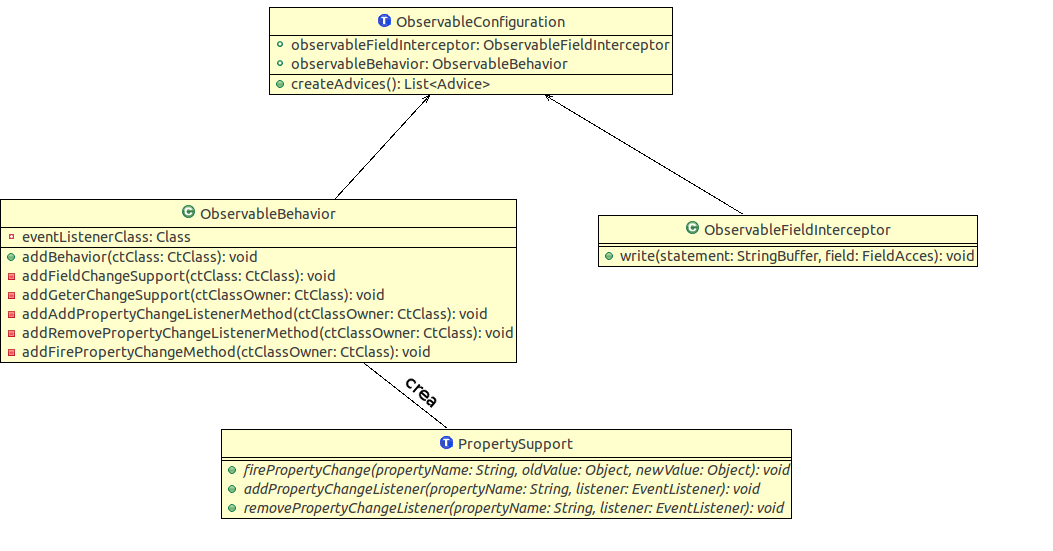
\includegraphics[scale=0.45]{img/poo}
	 	\caption{Esquema de la herramienta POO}
	 	\label{umlpoo}
	\end{figure}
	